\chapter{Transmission lines}\label{lec:lec2}
Transmission lines are special cases of electromagnetic waves that deal solemnly with time-varying voltage and current. In the previous chapter, emphasis was placed on the subject of electromagnetic waves that deal with electric and magnetic fields that vary with time. Transmission lines are unique because the concept of voltage and current are still very much valid.

In this chapter, we will still be working with the concept of voltage and current which everyone is familiar with and then gradually introduce the concept of space into the circuit analysis. 

\section{Structures of transmission lines}
Transmission lines can best be defined as a medium of power transfer from one point to another, this transmission is done through a variety of structures, some of which are explained below;

\subsection{Co-axial cable}	
\begin{figure}[h]
\centering
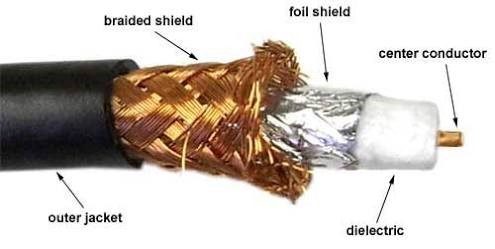
\includegraphics[scale=0.65]{./graphics/coaxial}
\caption{Co-axial cable transmission line}
\end{figure}
 In this particular setup, there’s an inner and outer conductor and voltage is applied between the inner and outer conductor thus energy will be propagated along the length of the structure.
\subsection{Parallel wire transmission lines}
 \begin{figure}[h]
\centering
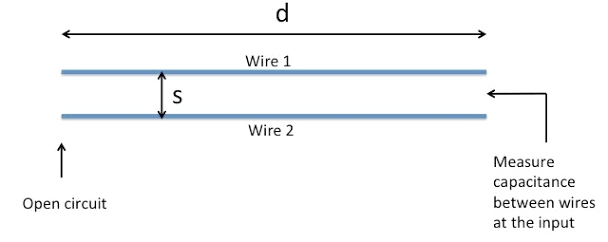
\includegraphics[scale=0.4]{./graphics/twowire}
\caption{Parallel wire}
\end{figure}
This setup is quite the simplest. We simply have two separate conductors hence when voltage is applied at both ends, energy flows.
\subsection{Microstripline}
\begin{figure}[h]
\centering
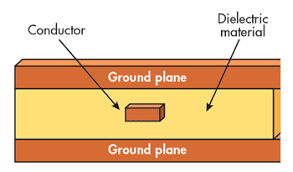
\includegraphics[scale=0.7]{./graphics/micro}
\caption{Microstripline }
\end{figure}
The microstrip line is a transmission line geometry with a single conductor trace on one side of a dielectric substrate and a single ground plane on the other side.
\subsection{Unbalanced}
\begin{figure}[h]
\centering
\includegraphics[width=1\linewidth]{./graphics/Unbalanced}
\caption{ Unbalanced }
\end{figure}
 In this structure we have a conducting rod above a ground surface and voltage is applied between the rod and the ground surface hence power is transmitted efficiently along the structure.
\subsection{Stripline} 
Also known as differential-stripline. The structure is made up of two parallel conductors enmeshed in a dielectric that has conducting surfaces at the top and bottom which are grounded while the voltage is applied between the two conductors.
\begin{figure}[h]
\centering
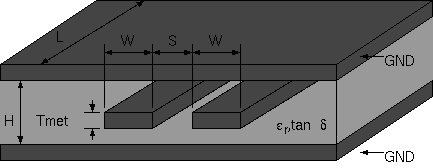
\includegraphics[width=1\linewidth]{./graphics/stripline}
\caption{ Stripline}
\end{figure}

The summary of all we have been discussing is that we are having a two-conductor system, hence when voltage is applied between them. Because it is a time-varying voltage current that flows through the system.

All the structures can be represented by a simple two-conductor system and this is also done for transmission line analysis where we ignore the structure and simply treat it as a two-conductor system, at one end we apply an energy source and at the other end, we apply a load and then carry out analysis from the source to the load.

\section{Concept of transit time effect }
Circuit laws like Kirchhoff’s law, are limited to low-frequency circuits where we only take note of the value of the electrical components, i.e. For a circuit that comprises resistors, capacitors and inductors, only their values are needed for the circuit analysis.

However, as frequency increases, the signal value changes significantly. A good example is shown in Figure~\ref{fig:first}.

\begin{figure}[h]
\centering
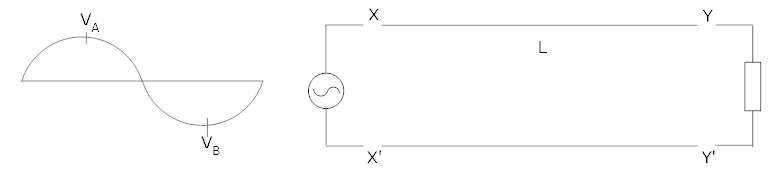
\includegraphics[width=1\linewidth]{./graphics/first}
\caption{circuit diagram of a transmission line}
\label{fig:first}
\end{figure}

At some instant, $ V_{A} $ is applied at X, and when L is sufficiently small relative to the length ($  \lambda = \text{wavelength} $). We assume that $ V_{A} $ appears at Y from X almost instantaneously.

But if $f$ (frequency) of the signal is very high, $\lambda $ gets very small and so is far less than L, hence  $  V_{A} $ applied at X takes some finite time before It gets to Y as $  L\gg \lambda $ (high frequency). Therefore $  V_{Y} $ is not always $  V_{X} $.

In transit time effect one can realise that $ \lambda $  approaches L and so it is very likely that $ V_{X} \neq V_{Y} $, but when $  \lambda \gg L  $ (for low-frequency circuits) the sinusoidal wave changes slowly so that we can assume it is constant across the entire L.\\
The finite time it takes the voltage at X to appear at Y is called transit time.
\begin{align}
 t_{r} = \frac{L}{v}\ \ \ \ \ \ (\text{Transit  Time})
\end{align}
$v$ is the velocity of the signal. So when a time-varying signal is applied at X, it requires a finite time to travel from X to Y.  $ V_{A} $  at X will not remain constant as it is a time-varying sinusoidal so that in the transit time it takes $ V_{A} $ to appear at Y, $ V_{A} $ would have changed to another value say $ V_{B} $, so when a voltage at Y is $ V_{B} $ say, the voltage at X is $ V_{A} $. In other words, there is a potential difference between X and Y. This difference is related to the length of the cable, the more the length the more the difference, with L very small. $ V_{x} $ is close to $ V_{y} $ as the points A and B will be close to each other and the voltage difference will not be substantial. The important thing here is no matter how small the length we take, there will always be that voltage difference $ V_{x} – V_{y} = 0 $ if $ L \rightarrow 0 $.

As we increase the frequency, the role of the transit time effect becomes more and more important. So now to the big question; \textit{When do you neglect transit time effect and when do you incorporate it in your design?}

If $ V_{x} – V_{y} $ is small, the transit time effect can be neglected otherwise it should be taken into consideration. Generally, if  $ t_{r} \ll T $ (period of signal) neglects transit time effect but if $ t_{r} $ is comparable to T (signal period), then we have to incorporate the effect of transit time in other words, when carrying out circuit analysis, the size of the structures has started playing a role in the analysis.
$$ T \gg t_{r}\ \ \ \ \ \ (\text{neglect transit time})$$\\\\
 Recall T = $   \frac{1}{f}  $, $ t_{r} = \frac{L}{v} $ and $ \lambda = \frac{v}{f} $\ \ \ \ \ \ hence; 

$ \frac{1}{f} \gg \frac{L}{v} $ or $ \frac{v}{f} \gg L $ \\\\
Thus, $ \lambda \gg L $ \ as a result, the transit time effect is neglected.

\section{Analysis of Transmission line}
In low-frequency analysis, there is just a circuit size that fits all values like saying R= $ 0.1\Omega $, L=0.1H and C = $ 0.1\mu F $, unlike in high frequency where we have $ 10\Omega $ resistor of 1cm, 10cm and 100cm lengths which will cause each of the circuit to behave differently because of the non-uniform length when transit time effect is considered.

However, we still want to use the basic laws that we are familiar with for low frequency. The approach of this law will break the\textbf{ LUMPED ELEMENT} into \textbf{DISTRIBUTED ELEMENT} and also have per unit element value for each of the elements. The division of each circuit element in space is done in such a way that L is infinitesimally small so that the circuit laws at low frequency can apply within two nodes created by the division.\\

Transit time cannot be neglected for a two-conductor wire but when a small quantity in length is broken down into very Lineal elements of $ \Delta x $ with  $  \Delta x \rightarrow 0 $. The transit can be neglected as $ L \gg \Delta x $ and so the circuit laws of low frequency can be applied to the arbitrary nodes separated by $ \Delta x $ length. \\
In the circuit, we should have resistance, capacitance and inductance stated in total value, instead, we have resistance, inductance and capacitance all per unit length.

The relationship between voltage and current is valid for high frequency like that of low frequency as $ \Delta x  \rightarrow 0$ (infinitesimally small). Hence, this solves for voltage and current of a transmission line in the presence of the transit time effect.\\
\begin{figure}[h]
\centering
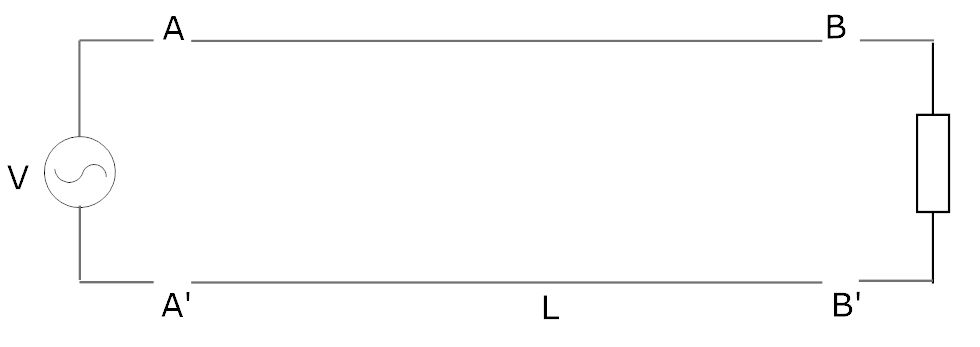
\includegraphics[width=1\linewidth]{./graphics/second}
\caption{simple circuit diagram of a transmission line}
\end{figure}	

In the circuit above, there is a voltage difference between both ends because of the transit time effect but we do not know why there is a voltage difference.

We all know that as frequency increases in the circuit, the two conductors have both electric and magnetic fields induced as shown below: 

\begin{figure}[h]
\centering
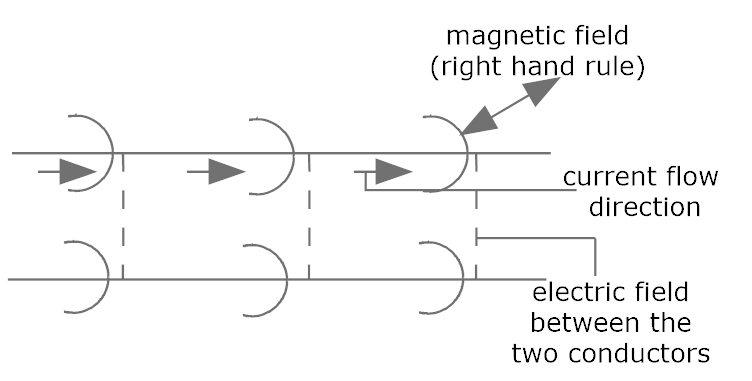
\includegraphics[width=1\linewidth]{./graphics/third}
\caption{transmission line circuit showing both electric and magnetic fields}
\end{figure}

So when the magnetic field is linked with current an inductance is produced while the electric field between the two conductors with air as dielectric gives a capacitor.

\begin{figure}[h]
\centering
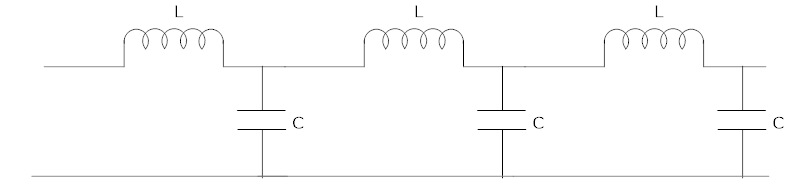
\includegraphics[width=1\linewidth]{./graphics/fifth}
\caption{distributed inductance and capacitance in transmission line circuit}
\end{figure}
The inductance and capacitance produced are distributed along the length of the structure. These parameters are called the \textbf{Distributed Parameters of the Line.} \\
At low frequency, there is no voltage drop across the length of a transmission line but as frequency starts to increase, the reactance of inductor $ (X_{l} $) starts causing a voltage drop across the length of the transmission line that was not seen at low frequency.
\[ 	X_{l} = 2 \pi FL \]
Hence, from a finite time point of view, there is a potential difference as a result of the transit time effect. Conductors do not have zero resistance and the separation of the conductor as a dielectric is not ideal so the current flow between the conductor across the conductance of the dielectric.\\

Hence, we have a more realistic transmission line modelled as;\\
\begin{figure}[h]
\centering
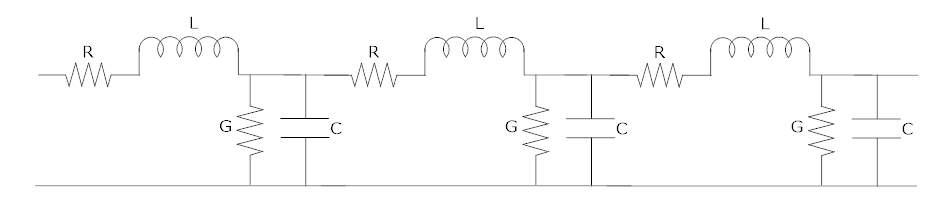
\includegraphics[width=1\linewidth]{./graphics/sixth}
\caption{Distributed elements for lossless transmission}
\end{figure}
In the diagram above, the resistance, capacitance, inductance and conductance are all per unit length values. We have defined the quantities which are called the PRIMARY CONSTANT of the transmission line which is;\\\\
Resistance per unit length – Ohms/metre\\
Inductance per unit length – Henry/metre\\
Capacitance per metre – Farad/metre\\
Conductance per metre – Siemens/metre\\

After the primary constants have been determined then the analysis of the transmission line can be carried out by;
\begin{enumerate}
\itemsep0em
\item Dividing the transmission line into small segments.
\item Writing down Kirchoff's law of voltage and current for the segment.
\item Carry out the analysis when the segment goes to zero to enable the analysis to be valid for any high frequency or any low wavelength. 
\item Apply voltage to the segment that causes current to flow into the circuit.
\end{enumerate}
\begin{figure}[h]
\centering
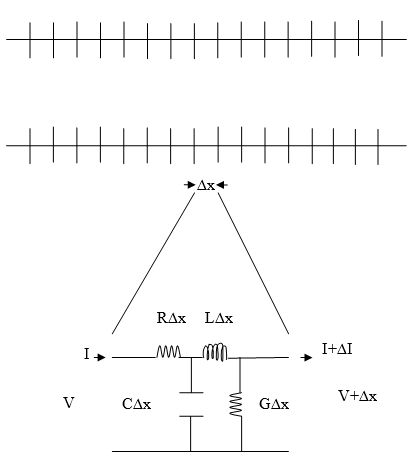
\includegraphics[scale=0.4]{./graphics/seventh}
\caption{circuit analysis of a small segment of the transmission line}
\end{figure}
Since the segment is very small and voltage has an angular frequency $ \omega $ then;
\begin{align}  
\Delta V = - (R \Delta x + j\omega L\Delta x)I
\label{eqn:voltage}
\end{align}
\begin{align}
\Delta I = - (G \Delta x + j \omega C \Delta x)V
\label{eqn:current}
\end{align}
We notice a negative sign in $ \Delta I $ and $ \Delta V $ expression which is because as we move in the direction of current flow there is a drop in voltage that will make (I +$  \Delta I $) and (v + $ \Delta V) $ values lesser than I and V at the start node.

For equations \ref{eqn:voltage} and \ref{eqn:current} to be valid at all frequencies, $ \Delta x $ must tend to zero.\\
From equation~\ref{eqn:voltage} we have;
\[ \Delta V = - (R \Delta x + j\omega L\Delta x)I \]
\[ \Delta V = - (R + j\omega L)\Delta x I \]

\[ \frac{	\Delta V }{\Delta x} = \frac{ - (R  + j\omega L)\Delta x I}{\Delta x} \]

\[ \frac{	\Delta V }{\Delta x} =  - (R  + j\omega L) I \]

\[ \lim_{ \Delta x\to 0} \frac{\Delta V}{ \Delta x} = \frac{ dV}{ \ dx} = - (R + j \omega L)I \]
 \begin{align}
\frac{ dV}{ \ dx} = - (R + j \omega L)I 
\label{eqn:deltav}
 \end{align} 
Also, from equation~\ref{eqn:current} we have,
\[ \Delta I = - (G \Delta x + j\omega C\Delta x)V \]
\[ \Delta I = - (G + j\omega C)\Delta x V \]

\[ \frac{	\Delta I }{\Delta x} = \frac{ - (G + j\omega C)\Delta x V}{\Delta x} \]
   
\[ \frac{	\Delta I }{\Delta x} =  - (G + j\omega C) V \]
   
\[ \lim_{ \Delta x\to 0}	\frac{ \Delta I}{ \Delta x} = \frac{dI}{dx} = - (G + j\omega C)V \]
\begin{align}
\frac{dI}{dx} = - (G + j\omega C)V 
\label{eqn:deltai}
\end{align}
Equations \ref{eqn:deltav} and \ref{eqn:deltai} are said to be \textbf{Coupled Equations} since $ \frac{dV}{dx} $ is related to $I$ and $ \frac{dI}{dx} $  is related to $V$.

Hence, we see that the voltage and current as $ \Delta x \rightarrow $ 0 are not related by algebraic equations but by a differential equation.\\
By differentiating equations \ref{eqn:deltav} and \ref{eqn:deltai} again, we have; 
\begin{align}
\frac{d^{2}V}{dx^{2}} = - (R + j\omega L)\frac{dI}{dx} 
\label{eqn:delta2v}
\end{align}
\begin{align}
\frac{d^{2}I}{dx^{2}} = - (G + j\omega C)\frac{dv}{dx}
\label{eqn:delta2i}
\end{align}
Substituting equation \ref{eqn:delta2v} into \ref{eqn:delta2i} we have,
\[ 	\frac{d^{2}V}{dx^{2}} = - (R + j\omega L)\times {- (G + j\omega C)V} \]
\begin{align}
 \frac{d^{2}V}{dx^{2}} = (R + j\omega L)(G + j\omega C)V 
\label{eqn:deqn}
\end{align}   
\\
The coefficient of V in equation~\ref{eqn:deqn} must be a primary quantity of the transmission line since it depends on the primary constant of the transmission line and the frequency of operation $ \omega$. Let's call the quantity $ \gamma^{2}. $ 

Therefore, 
\begin{align}
\frac{d^{2}V}{dx^{2}} = \gamma^{2}V 
\label{eqn:deqnv}
\end{align}
\begin{align}
\frac{d^{2}I}{dx^{2}} = \gamma^{2}I 
\label{eqn:deqni}
\end{align}
Equations \ref{eqn:deqnv} and \ref{eqn:deqni} are referred to as the \textbf{Telegraphers Equation}.

These are now the voltage and current expressions that governs a transmission line. The quantity $ \gamma $ is called the \textbf{Propagation Constant}. The quantity $V$ and $I$ are sinusoidal and so vary with $ e ^{j\omega t}$. The quantity $ e ^{j\omega t} $ helps take care of the harmonic time variation in V an I. \\
Since $ \gamma $ is a constant for a given line and frequency, 
\[ \frac{d^{2}V}{dx^{2}} = \gamma^{2}V\]\\
Therefore; 
\begin{align}
V(x) = V^{+} e ^{- \gamma x} + V^{-}e^{\gamma x}  
\label{eqn:solnv}
\end{align}
$ 	V(x) = V^{+} e ^{- \gamma x} + V^{-}e^{\gamma x} $  is the RMS or peak value. 

To find the instantaneous value of $V$, we multiply equation~\ref{eqn:solnv} by $ e ^{j\omega t}$.  V depends on $x$ and $t$. So,
\[ 	V(x,t) = V^{+} e^{-\gamma x}e^{j\omega t} + V^{-} e^{\gamma x}e^{j\omega t} \]
The only way to show the amplitude and the initial phase is through a complex number. therefore,

$ V^{+} $= Complex value of voltage at x= 0 location with a certain initial phase. Hence why V is always complex;

\[ 	V(x,t) = V^{+} e^{-\gamma x}e^{j\omega t} + V^{-} e^{\gamma x}e^{j\omega t} \]

But $ \gamma = \alpha + j\beta $	 is also a complex quantity. 
\[ V^{+}e^{- \gamma x}e^{j \omega t} = V^{+}e^{-( \alpha + j \beta )x}e^{j \omega t} = V^{+}e^{-\alpha x}e^{j(\omega t - \beta x)}
 \]

$ V^{+}e^{-\alpha x} $ is a voltage whose amplitude varies exponentially along the transmission line and the phase of the voltage is a combination of space and time from $  (\omega t- \beta x) $, $ \omega t $ from time and $ \beta x  $ from space. Hence $ V^{+}e^{-\gamma x}e^{jwt} \equiv V^{+}e^{-\alpha x}e^{j( \omega t-\beta x)} $ is the first point of V(x,t) and represent something whose amplitude varies along the length and the phase of which is a combination of space and time.\\

For understanding say, $  V^{+} $ is real and positive and $ \alpha= 0 $ then
\begin{align*}
V^{+}e^{-\alpha x}e^{j( \omega t-\beta x)} = V^{+} e^{j( \omega t-\beta x)}
\end{align*}
We plot this as a function of space and time
 \[ V^{+}e^{j( \omega t-\beta x)} = V^{+}cos(\omega t- \beta x) +  V^{+}jsin(\omega t- \beta x)\footnote{Recall from Euler's formula; $ e^{j\theta} = cos\theta + jsin\theta $}\]

Since we want real voltage we take only $ V^{+}cos(\omega t- \beta x) $ and plot variation of $ V $ with respect to $ x $ and $ t $. We have the graph shown below for different $ t $, as $ t $ increases, a point in the plot moves rightward. Hence with respect to space and time, the graph moves rightward as time increases. This is called a \textbf{Travelling wave phenomenon}.

\begin{figure}[h]
\centering
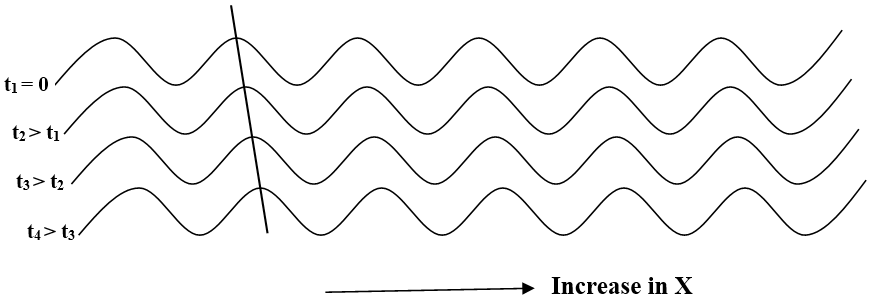
\includegraphics[width=1\linewidth]{./graphics/ABC}
\caption{Voltage as a function of X for different time}
\end{figure}
Hence  $ V^{+}e^{j(\omega t- \beta x )} $ is a positive or progressive travelling wave as it moves rightward with an increase in time. Similarly, when $ V^{-}e^{j( \omega t+ \beta x )} $ is plotted on the graph, the point starts moving leftward with an increase in time and it is called \textbf{negative travelling wave}.

\begin{figure}[h]
\centering
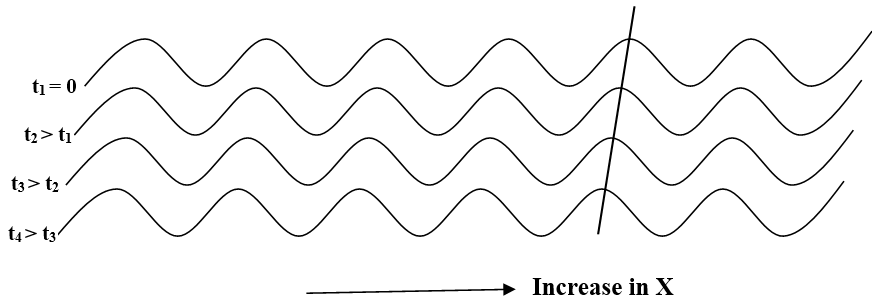
\includegraphics[width=1\linewidth]{./graphics/ABCD}
\caption{Voltage as a function of X for different time}
\end{figure}

Hence with high-frequency circuit analysis, the voltages and current have to be visualized in the form of waves. 

In conclusion, we see that a departure from the lumped element analysis to the distributed circuit analysis radically changes the approach to circuit analysis to a voltage and current that exist in the form of waves on the electrical circuits. 